\begin{BPMN}{PROC-02}{Creación de una Unidad de Aprendizaje}{}
    \PCitem{Participantes}{\begin{itemize}
    		\item Docentes de la Academias	
    		\item Comité de Evaluación Curricular
    		\item Colegio de Profesores
    		\item Dirección General 
    \end{itemize}}
    \PCitem{Objetivo}{La elaboración o rediseño  de las Unidades de Aprendizaje, ya sea de forma individual o en paquetes, que pertenecen a un Plan de Estudios en un Programa Académico del IPN.}
    \PCitem{Interrelación con otros procesos}{
    \begin{itemize}
    	\item Entrada: Requisito de rediseñar o diseñar una nueva Unidad de Aprendizaje en un Plan de Estudios.
    	\item Salida: Tiras de Unidades de Aprendizaje en un Plan de Estudios.
	\end{itemize}
}
    \PCitem{Proveedores}{Dirección de Educación Superior}
    \PCitem{Entradas}{Plantillas de creación de Unidades de Aprendizaje}
    \PCitem{Consumidores}{Unidad Académica}
    \PCitem{Salidas}{Tiras de unidades de aprendizaje}
    \PCitem{Precondiciones}{Carga de resumen del Plan de Estudios}
    \PCitem{Postcondiciones}{Finalización del diseño o rediseño de un Programa Académico}
    \PCitem{Frecuencia}{Cuando se genera  un propuesta de creación o rediseño}
    \PCitem{Tipo}{Operativo}
    \PCitem{Áreas de oportunidad}{Actualización de las Unidades de Aprendizaje en un Plan de Estudios}
\end{BPMN}
En la figura \hyperref[fig:BPMN-02]{BPMN-02 Proceso para la creación de una Unidad de Aprendizaje}

\begin{figure}[htbp]
	\begin{center}
		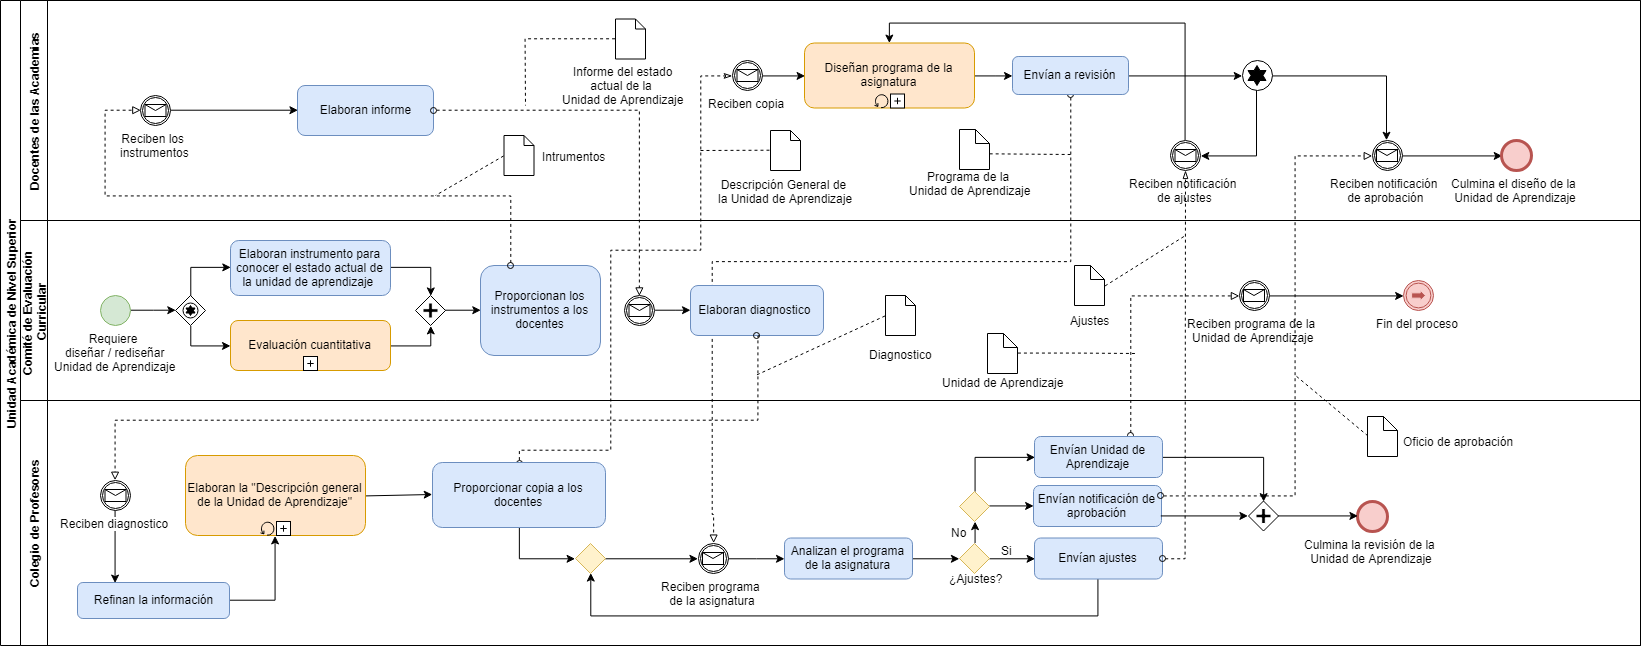
\includegraphics[width=.80\textwidth]{C1-DP/SP1/IG-SP1/BPMN-02}
		\caption{BPMN-02 Proceso para la creación de una Unidad de Aprendizaje}
		\label{fig:BPMN-02}
	\end{center}
\end{figure}
\newpage
\begin{itemize}
	\item \textbf{Elaborar instrumento para conocer el estado actual de la unidad de aprendizaje:} Se realiza la evaluación curricular dentro de la Unidad Académica para determinar la viabilidad de actualizar la Unidad de Aprendizaje.
	\item \textbf{Evaluación cuantitativa:}
	\item \textbf{Proporcionar instrumentos a los docentes:} Enviar los instrumentos y resultados de la evaluación curricular a los docentes encargados de la realización de la Unidad de Aprendizaje.
	\item \textbf{Elaborar informe:} Los docentes encargados, con base a los resultados obtenidos en la evaluación, realizan el informe del estado actual de la Unidad de Aprendizaje.
	\item \textbf{Elaborar diagnóstico:} Se determina si se aprueba o se rechazan los procesos de diseño o rediseño de la Unidad de Aprendizaje, según el informe del estado actual y la evaluación realizada.
	\item \textbf{Elaborar la "Descripción general de la Unidad de Aprendizaje":} Iniciar los procesos de rediseño o diseño de la Unidad de Aprendizaje. Se describe la asignatura.
	
	\item \textbf{Diseñar el programa de la asignatura:} Se inician los procesos de llenado de los programas sintéticos y en extenso de la Unidad de Aprendizaje.
	\item \textbf{Enviar a revisión:}  Los docentes envían los programas de la asignatura al Colegio de Profesores para su revisión.
	\item \textbf{Analizar el programa de la asignatura:} Se inician los trabajos de revisión de los programas sintéticos y en extenso de la Unidad de Aprendizaje por parte del Colegio de Profesores.
	
	\item \textbf{Enviar Unidad de Aprendizaje:}  Una vez aprobados los programas de la Unidad de Aprendizaje, se envían al Comité de Evaluación Curricular. Culmina el proceso.
	\item \textbf{Enviar ajustes:} Si existen correcciones o notas respecto a los programas de la Unidad de Aprendizaje, éstos se envían junto a ésta de vuelta a los docentes para ser atendidos.    
	 
	 
	

\end{itemize}